\chapter{GUI编程}

\section{GUI编程}

\subsection{GUI编程}

图形用户接口GUI(Graphic User Interface)是人机交互的重要技术手段,利用GUI技术可以方便使用者使用。在不同的编程语言内部实际上也提供有一系列GUI组件。\\

如果要编写出一个图形界面,就必须非常清楚每一种组件的定义及相关的处理操作,同时还需要清除整个界面组件的布局管理。在Python中可以使用tkinter、Pyqt5组件,如果有Java的开发能力,也可以使用Jython通过Java语言类库实现图形化界面开发。在tkinter模块中提供了多种不同的窗体组件:

\begin{table}[H]
	\centering
	\setlength{\tabcolsep}{5mm}{
		\begin{tabular}{|c|l|}
			\hline
			\textbf{组件} & \textbf{描述}                        \\
			\hline
			Button        & 按钮                                 \\
			\hline
			Checkbutton   & 多选框                               \\
			\hline
			Entry         & 输入框                               \\
			\hline
			Frame         & 框架控件,在进行排版时实现子排版模型 \\
			\hline
			Label         & 标签                                 \\
			\hline
			Listbox       & 列表框                               \\
			\hline
			Menu          & 菜单                                 \\
			\hline
			Menubutton    & 菜单按钮,为菜单定义菜单项           \\
			\hline
			Radiobutton   & 单选按钮                             \\
			\hline
			Scale         & 滑动组件                             \\
			\hline
			Scrollbar     & 滚动条组件                           \\
			\hline
			Text          & 文本                                 \\
			\hline
			LabelFrame    & 容器组件,实现复杂组件布局           \\
			\hline
			tkMessageBox  & 消息组件,可以进行提示框的显示       \\
			\hline
		\end{tabular}
	}
	\caption{tkinter模块窗体组件}
\end{table}

\vspace{0.5cm}

\subsection{窗体}

任何一个图形界面都包含一个主窗体,在主窗体内可以设置不同的组件。tkinter模块中提供了Tk类,负责窗体的创建以及相关的属性定义。\\

\begin{table}[H]
	\centering
	\setlength{\tabcolsep}{4mm}{
		\begin{tabular}{|l|l|}
			\hline
			\textbf{方法}                               & \textbf{功能}            \\
			\hline
			title(self, string=None)                    & 设置窗体显示标题         \\
			\hline
			iconbitmap(self, bitmap=None, default=None) & 设置窗体logo             \\
			\hline
			geometry(self, newGeometry=None)            & 设置窗体大小             \\
			\hline
			minsize(self, width=None, height=None)      & 设置窗体最小化尺寸       \\
			\hline
			maxsize(self, width=None, height=None)      & 设置窗体最大化尺寸       \\
			\hline
			mainloop(self, n=0)                         & 界面循环及时显示窗体变化 \\
			\hline
		\end{tabular}
	}
	\caption{Tk类}
\end{table}

mainloop()的主要作用是进行窗体的显示,所有的窗体都是基于绘图的原理绘制的,所以调用此方法表示窗体进行持续的状态的显示变化。\\

\mybox{创建窗体}

\begin{lstlisting}[language=Python]
import tkinter

class MainForm:
    """
        窗体类
    """
    def __init__(self):
        self.root = tkinter.Tk()         # 创建窗体
        self.root.title("GUI编程")
        self.root.geometry("500x200")    # 初始化窗口尺寸
        self.root.maxsize(1000, 400)     # 最大尺寸
        self.root["background"] = "LightSlateGray"   # 浅青灰色
        self.root.mainloop()             # 显示窗体

def main():
    MainForm()

if __name__ == "__main__":
    main()
\end{lstlisting}

\begin{tcolorbox}
	\mybox{运行结果}
	\begin{figure}[H]
		\centering
		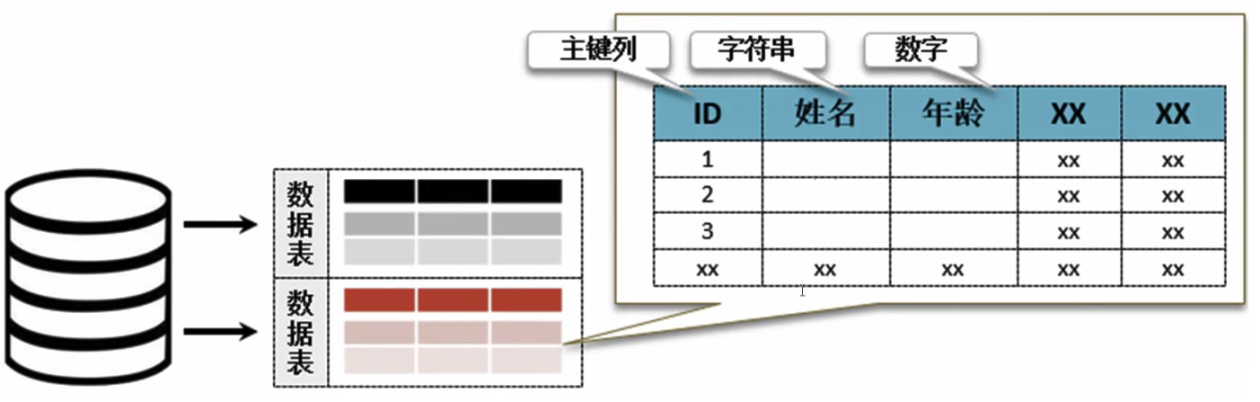
\includegraphics[]{img/C13/13-1/1.png}
	\end{figure}
\end{tcolorbox}

\vspace{0.5cm}

\subsection{基础控件}

在tkinter模块中提供了Label组件类。在一个窗体中如果要定义一些提示文字信息就可以利用标签。\\

所有的GUI组件一定要在窗体上进行各种配置,而每个组件本身有需要进行布局。如果标签没有进行布局的控制,就会按照基本的样式进行显示处理。\\

为了方便人机交互,基本都要求有一个文本输入。在tkinter模块中提供有Text组件类,这个类的最大特点就是可以进行单行文本、多行文本、图片、HTML代码的显示处理能力。\\

按钮是在图形界面之中最为常见的指令发送组件,在图形界面之中往往都是通过Text文本组件进行文字内容的输入,而后利用按钮进行相应的处理。在tkinter模块中使用Button可以实现按钮的定义。\\

\mybox{基础控件}

\begin{lstlisting}[language=Python]
import tkinter

class MainForm:
    def __init__(self):
        self.root = tkinter.Tk()
        self.root.title("GUI编程")
        self.root.geometry("500x200")

        # 标签
        self.label = tkinter.Label(
            self.root, text="用户名",
            width=10, height=5,
            font=("微软雅黑", 14)
        )

        # 文本
        self.text = tkinter.Text(
            self.root, width=20, height=1,
            font=("微软雅黑", 12)
        )
        self.text.insert(tkinter.CURRENT, "输入用户名")

        # 按钮
        self.button = tkinter.Button(self.root, text="登录")

        # 组件布局
        self.label.pack(side="left")
        self.text.pack(side="left")
        self.button.pack(side="left")

        self.root.mainloop()

def main():
    MainForm()

if __name__ == "__main__":
    main()
\end{lstlisting}

\begin{tcolorbox}
	\mybox{运行结果}
	\begin{figure}[H]
		\centering
		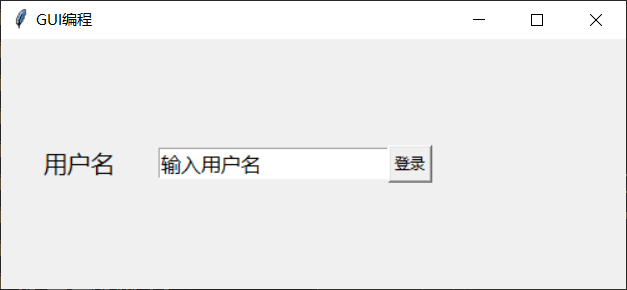
\includegraphics[]{img/C13/13-1/2.png}
	\end{figure}
\end{tcolorbox}

\newpage

\section{事件}

\subsection{事件}

图形界面中除了组件的基本展示之外,最为重要的就是要定义与组件有关的事件处理操作。在tkinter中可以方便地为每一个组件进行事件绑定,并且设置事件的相关处理函数,这样每当触发相应的事件之后就可以通过特定地函数实现事件处理。

\begin{figure}[H]
	\centering
	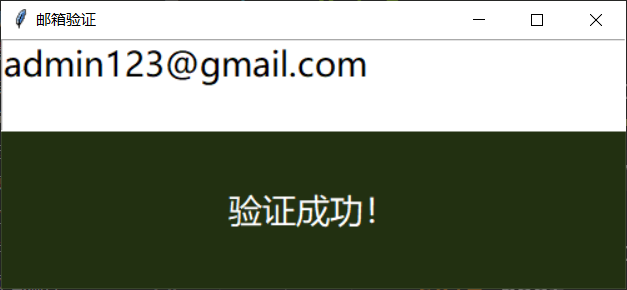
\includegraphics[]{img/C13/13-2/1.png}
\end{figure}

当事件触发后会产生一个事件对象,利用这个事件对象可以在处理函数中获得相应的数据信息,例如哪一个组件触发的操作、操作的坐标等。\\

通过使用bind()可以进行事件的绑定,而在绑定的时候一定要有每一个方法对应的事件的类型,事件的类型是由tkinter规定好的。

\begin{table}[H]
	\centering
	\setlength{\tabcolsep}{5mm}{
		\begin{tabular}{|c|l|}
			\hline
			\textbf{事件} & \textbf{功能}                  \\
			\hline
			Button        & 当用户点击鼠标按键时触发       \\
			\hline
			ButtonRelease & 鼠标按键松开时触发             \\
			\hline
			Enter         & 当鼠标指针进入组件时触发       \\
			\hline
			FocusIn       & 当组件获得焦点时触发           \\
			\hline
			FocusOut      & 当组件失去焦点时触发           \\
			\hline
			KeyPress      & 当键盘按下时触发               \\
			\hline
			KeyRelease    & 当按键松开时触发               \\
			\hline
			Leave         & 当鼠标指针离开组件时触发       \\
			\hline
			Motion        & 当鼠标在组件内部移动时触发     \\
			\hline
			Visibility    & 当应用组件可见时触发           \\
			\hline
			MouseWheel    & 当鼠标在组件内部滚轮滚动时触发 \\
			\hline
		\end{tabular}
	}
	\caption{事件}
\end{table}

\vspace{0.5cm}

\mybox{验证邮箱合法性}

\begin{lstlisting}[language=Python]
import  tkinter
import  re

#  合法邮箱正则语法
EMAIL  =  "[a-zA-Z0-9]\\w+@\\w+\\.(cn|com|com.cn|gov|net)"

class  MainForm:
    def  __init__(self):
        self.root  =  tkinter.Tk()
        self.root.title("邮箱验证")
        self.root.geometry("500x200")

        self.text  =  tkinter.Text(
            self.root,  width=500,  height=2,
            font=("微软雅黑",  20)
        )
        #  提示信息
        self.text.insert("current",  "输入邮箱")
        #  鼠标单击后删除文本组件中的全部内容
        self.text.bind("<Button-1>",  
            lambda  event:  self.text.delete("0.0",  "end"))
        #  绑定键盘事件
        self.text.bind("<KeyPress>",  
            lambda  event:  self.keyboard_event_handler(event))
        self.text.bind("<KeyRelease>",  
            lambda  event:  self.keyboard_event_handler(event))
        self.text.pack()

        self.content  =  tkinter.StringVar()      #  修改标签文字
        
        self.label  =  tkinter.Label(
            self.root,  width=200,  height=200,
            textvariable=self.content,
            bg="#223011",  fg="#ffffff",
            font=("微软雅黑",  20)
        )
        self.label.pack()

        self.root.mainloop()
    
    def  keyboard_event_handler(self,  event):
        """
            键盘处理时间
            Args:
                event:  事件
        """
        #  获取文本框数据
        email  =  self.text.get("0.0",  "end")
        if  re.match(EMAIL,  email):
            self.content.set("验证成功!")
        else:
            self.content.set("格式错误!")

def  main():
    MainForm()
    
if  __name__  ==  "__main__":
    main()
\end{lstlisting}

\begin{tcolorbox}
	\mybox{运行结果}
	\begin{figure}[H]
		\centering
		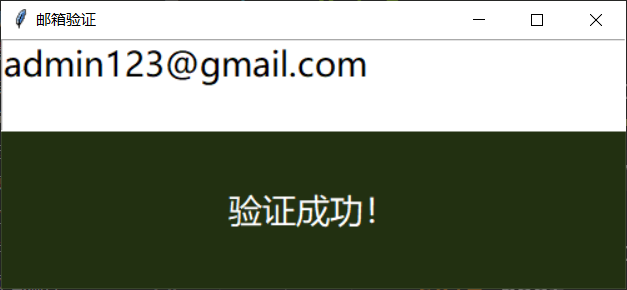
\includegraphics[]{img/C13/13-2/2.png}
	\end{figure}
\end{tcolorbox}

\newpage

\section{布局}

\subsection{pack布局}

pack布局是GUI布局之中最为常见的一种形式,这种布局属于顺序式排列布局。如果没有引入布局管理器的概念,实际上组件是不会显示的。如果没有对布局管理器进行合理的配置,显示的效果就会非常混乱。

\begin{table}[H]
	\centering
	\setlength{\tabcolsep}{3mm}{
		\begin{tabular}{|c|l|l|}
			\hline
			\textbf{参数} & \textbf{取值范围}                  & \textbf{功能}          \\
			\hline
			fill          & none、x、y、both                   & 是否水平或垂直方向填充 \\
			\hline
			expand        & yes(1)、no(0)                  & 是否可以展开           \\
			\hline
			side          & left、right、top、bottom           & 摆放位置               \\
			\hline
			anchor        & n、s、w、e、nw、ne、sw、se、center & 设置在窗体中八个方位   \\
			\hline
		\end{tabular}
	}
	\caption{pack布局}
\end{table}

\vspace{0.5cm}

\mybox{pack布局}

\begin{lstlisting}[language=Python]
import tkinter

class MainForm:
    def __init__(self):
        self.root = tkinter.Tk()
        self.root.title("GUI编程")
        self.root.geometry("500x200")

        label = tkinter.Label(
            self.root, text="用户名",
            width=10, height=2,
            font=("微软雅黑", 14)
        )
        text = tkinter.Text(
            self.root, width=20, height=2,
            font=("微软雅黑", 14)
        )
        text.insert("current", "输入用户名")

        label.pack(side="top")
        text.pack(side="bottom")
        self.root.mainloop()

def main():
    MainForm()

if __name__ == "__main__":
    main()
\end{lstlisting}

\begin{tcolorbox}
	\mybox{运行结果}
	\begin{figure}[H]
		\centering
		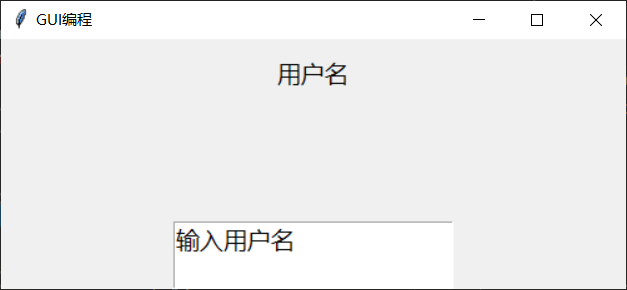
\includegraphics[]{img/C13/13-3/1.png}
	\end{figure}
\end{tcolorbox}

\vspace{0.5cm}

\subsection{grid布局}

grid布局利用表结构的形式来实现布局的管理,在一张数据表里面一定会有行和列,在使用grid布局的时候就可以通过行和列实现组件的摆放。\\

计算器实际上就属于一种grid布局的形式:

\begin{figure}[H]
	\centering
	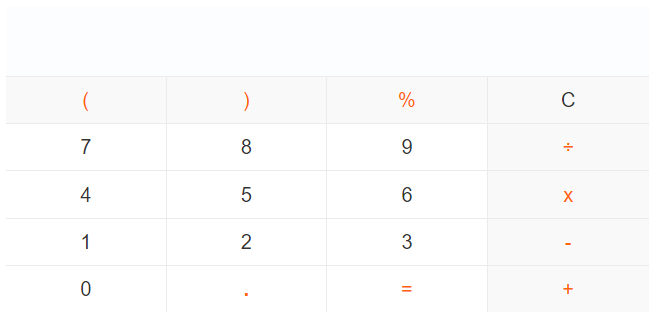
\includegraphics[]{img/C13/13-3/2.png}
	\caption{计算器}
\end{figure}

\vspace{0.5cm}

\mybox{grid布局}

\begin{lstlisting}[language=Python]
import tkinter

class MainForm:
    def __init__(self):
        self.root = tkinter.Tk()
        self.root.title("GUI编程")
        self.root.geometry("500x200")
        label1 = tkinter.Label(self.root, text="标签1")
        label2 = tkinter.Label(self.root, text="标签2")
        label1.grid(row=0, column=0)
        label2.grid(row=1, column=1)
        self.root.mainloop()

def main():
    MainForm()

if __name__ == "__main__":
    main()
\end{lstlisting}

\begin{tcolorbox}
	\mybox{运行结果}
	\begin{figure}[H]
		\centering
		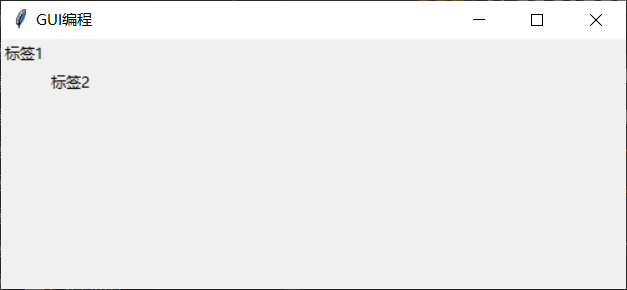
\includegraphics[]{img/C13/13-3/3.png}
	\end{figure}
\end{tcolorbox}

\vspace{0.5cm}

\subsection{place布局}

place布局是布局管理器之中最灵活的一种布局形式,它采用的是坐标点位置的布局操作。\\

\mybox{place布局}

\begin{lstlisting}[language=Python]
import tkinter

class MainForm:
    def __init__(self):
        self.root = tkinter.Tk()
        self.root.title("GUI编程")
        self.root.geometry("500x200")
        label = tkinter.Label(self.root, text="标签")
        label.place(x=100, y=50)
        self.root.mainloop()

def main():
    MainForm()

if __name__ == "__main__":
    main()
\end{lstlisting}

\begin{tcolorbox}
	\mybox{运行结果}
	\begin{figure}[H]
		\centering
		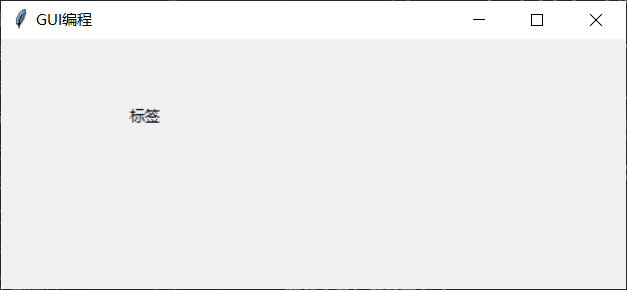
\includegraphics[]{img/C13/13-3/4.png}
	\end{figure}
\end{tcolorbox}

\vspace{0.5cm}

\subsection{Frame}

Frame是布局管理最为重要的一项布局技术,但是Frame本身并不是布局,而是一种内嵌的布局管理器。在一个窗体中针对不同的功能组件定义一个单独的区域,每一个区域相当于就是一个Frame,这些区域的内部都可以使用不同的布局管理器。

\begin{figure}[H]
	\centering
	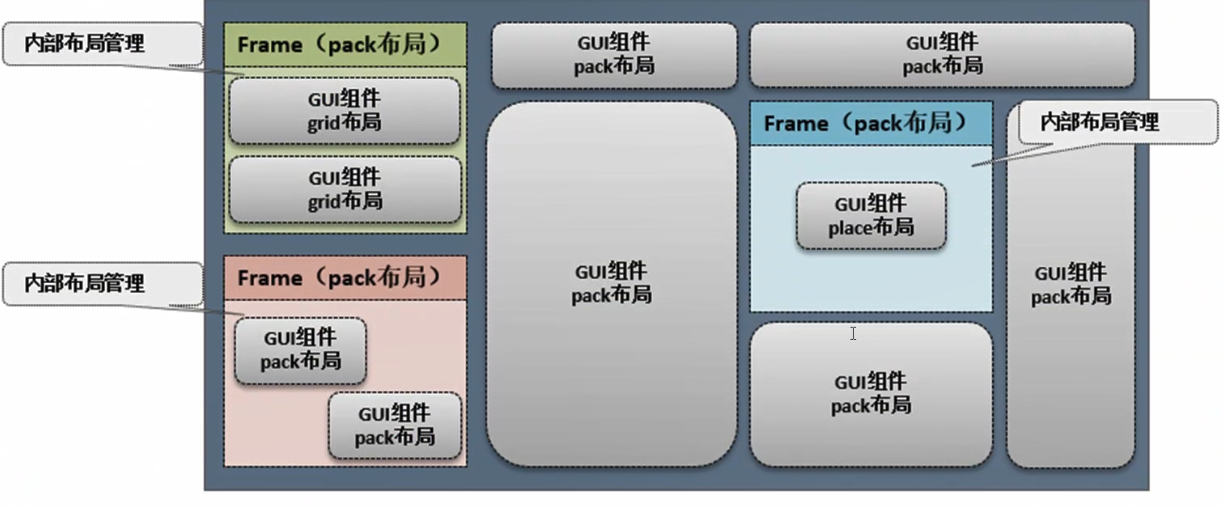
\includegraphics[scale=0.6]{img/C13/13-3/5.png}
\end{figure}

最具有代表性的Frame程序就是Windows中的计算器:

\begin{figure}[H]
	\centering
	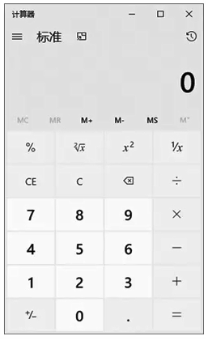
\includegraphics[]{img/C13/13-3/6.png}
	\caption{计算器}
\end{figure}

\vspace{0.5cm}

\mybox{计算器}

\begin{lstlisting}[language=Python]
import tkinter
import re

class MainForm:
    def __init__(self):
        self.root = tkinter.Tk()
        self.root.title("计算器")
        self.root.geometry("231x280")
        self.input_frame()      # 输入区
        self.button_frame()     # 按钮区
        self.root.mainloop()
    
    def input_frame(self):
        """
            输入区
        """
        # 创建内部容器
        self.in_frame = tkinter.Frame(self.root, width=20)
        self.content = tkinter.StringVar()
        # 单行输入
        self.entry = tkinter.Entry(
            self.in_frame, width=14,
            font=("微软雅黑", 20),
            textvariable=self.content
        )
        self.entry.pack(fill="x", expand=1)
        # 清除标记,每一次计算完成后清除
        self.clean = False
        self.in_frame.pack(side="top")
    
    def button_frame(self):
        """
            按钮区
        """
        self.btn_frame = tkinter.Frame(self.root, width=50)
        self.button_list = [[], [], [], []]     # 4行4列
        button = "123+456-789*0.=/"
        
        for row in range(4):
            for col in range(4):
                self.button_list[row].append(
                    tkinter.Button(
                        self.btn_frame,
                        text=button[4*row+col],
                        fg="black", width=3,
                        font=("微软雅黑", 20),
                    )
                )
        
        self.row = 0
        for group in self.button_list:
            self.column = 0
            for button in group:
                # 绑定事件
                button.bind(
                    "<Button-1>", 
                    lambda event: self.button_handler(event)
                )
                button.grid(row=self.row, column=self.column)
                self.column += 1
            self.row += 1
        self.btn_frame.pack(side="bottom")

    def button_handler(self, event):
        """
            按键事件处理
            Args:
                event: 单击事件
        """
        op = event.widget["text"]   # 获取按钮内容

        if self.clean:      # 新一次计算
            self.content.set("")    # 清除数据
            self.clean = False
        
        if op != "=":
            self.entry.insert("end", op)
        elif op == "=":
            result = 0
            expression = self.entry.get()
            pattern = r"\+|\-|\*|\/"

            nums = re.split(pattern, expression)
            op = re.findall(pattern, expression)[0]

            if op == "+":
                result = float(nums[0]) + float(nums[1])
            elif op == "-":
                result = float(nums[0]) - float(nums[1])
            elif op == "*":
                result = float(nums[0]) * float(nums[1])
            elif op == "/":
                result = float(nums[0]) / float(nums[1])
                
            self.entry.insert("end", "=%s" % result)
            self.clean = True

def main():
    MainForm()

if __name__ == "__main__":
    main()
\end{lstlisting}

\begin{tcolorbox}
	\mybox{运行结果}
	\begin{figure}[H]
		\centering
		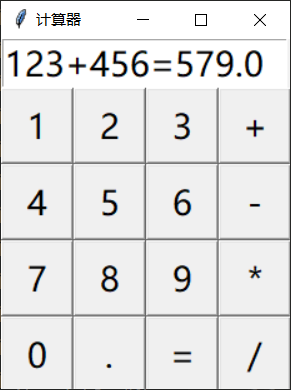
\includegraphics[]{img/C13/13-3/7.png}
	\end{figure}
\end{tcolorbox}

\newpage